% catalogue: title = Function plots with the plot path operation
% catalogue: min-coverage = 0.00
\documentclass[border=10pt]{standalone}
\PassOptionsToPackage{dvipsnames,svgnames,x11names}{xcolor}
\usepackage{tikz}
\usepackage{pgfplots}
\pgfplotsset{compat=newest}
\usepgfplotslibrary{groupplots}
\usetikzlibrary{arrows.meta}
\begin{document}
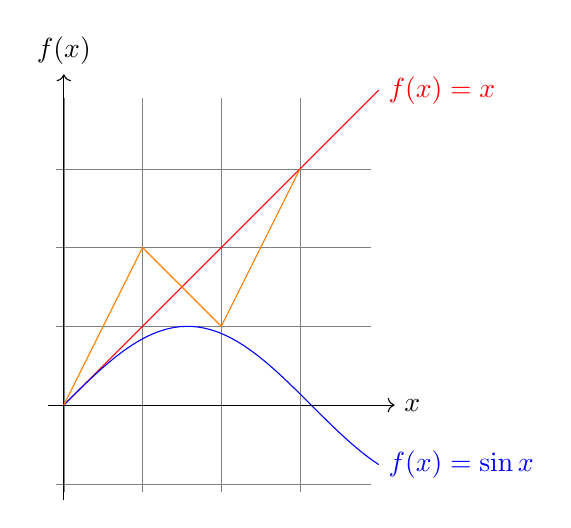
\begin{tikzpicture}[domain=0:4]
    \draw[very thin, color=gray] (-0.1, -1.1) grid (3.9, 3.9);
    \draw[->] (-0.2, 0) -- (4.2, 0) node[right] {$x$};
    \draw[->] (0, -1.2) -- (0, 4.2) node[above] {$f(x)$};
    \draw[color=red] plot (\x, \x) node[right] {$f(x) = x$};
    \draw[color=blue, samples=50] plot (\x, {sin(\x r)}) node[right] {$f(x) = \sin x$};
    \draw[color=orange] plot coordinates {(0, 0) (1, 2) (2, 1) (3, 3)};
\end{tikzpicture}
\end{document}
